\chapter{Resultados\label{chap:FundamentacaoMatematica}}

% Resumo opcional. Comentar se não usar.
%\resumodocapitulo{Resumo opcional.}

% Resumo informações da arquitetura relevantes do ponto de vista de controle
\section{Estudo Arquitetura}

Todo o código relacionado ao controle do robô é disponibilizado pelo fabricante e compôe a biblioteca M3, implementada em Python e com interface em C++. A partir da análise do código foi possível observar alguns pontos importantes que contribuem para ineficiência dos controladores implementado anteriormente:

\begin{itemize}
    \item Apenas controle por posição de juntas está implementado
    \item A taxa de atualização da memória compartilhada é de 100hz
\end{itemize}

Dentro do programa de interface com o ROS estão apenas definidos os controladores de posição com e sem compensação da gravidade. Os valores de velocidade e torque informados para o controle são completamente ignorados. Além disto a taxa de envio da informação obtida pelo ROS para a memória compartilhada é de apenas 100Hz definidos por hardcode. Foi feito um teste para alterar este valor para 1KHz porém o robô ficou completamente instável. De movo que novos testes não foram repetidos para evitar danos ao robô.

Este valor é bem próximo das taxas de amostragem de 8s (125 hz) e 20s (50 Hz) dos controladores implementados em C++ obtidas para os melhores resultados no trabalho feito pelo Marco Pereira. Sendo estes valores definidos pelo tempo mínimo necessário para efetuar todos os cálculos relacionados ao controladores cinemáticos implementados usando quatérnions duais.

\section{Estudo Controladores}

Foi observado que o controle do robô é feito a partir de uma série de controladores em cascata, conforme ilustrado no diagrama apresentado na figura \ref{fig:m3arch}.

\begin{figure}[H]
    \centering
    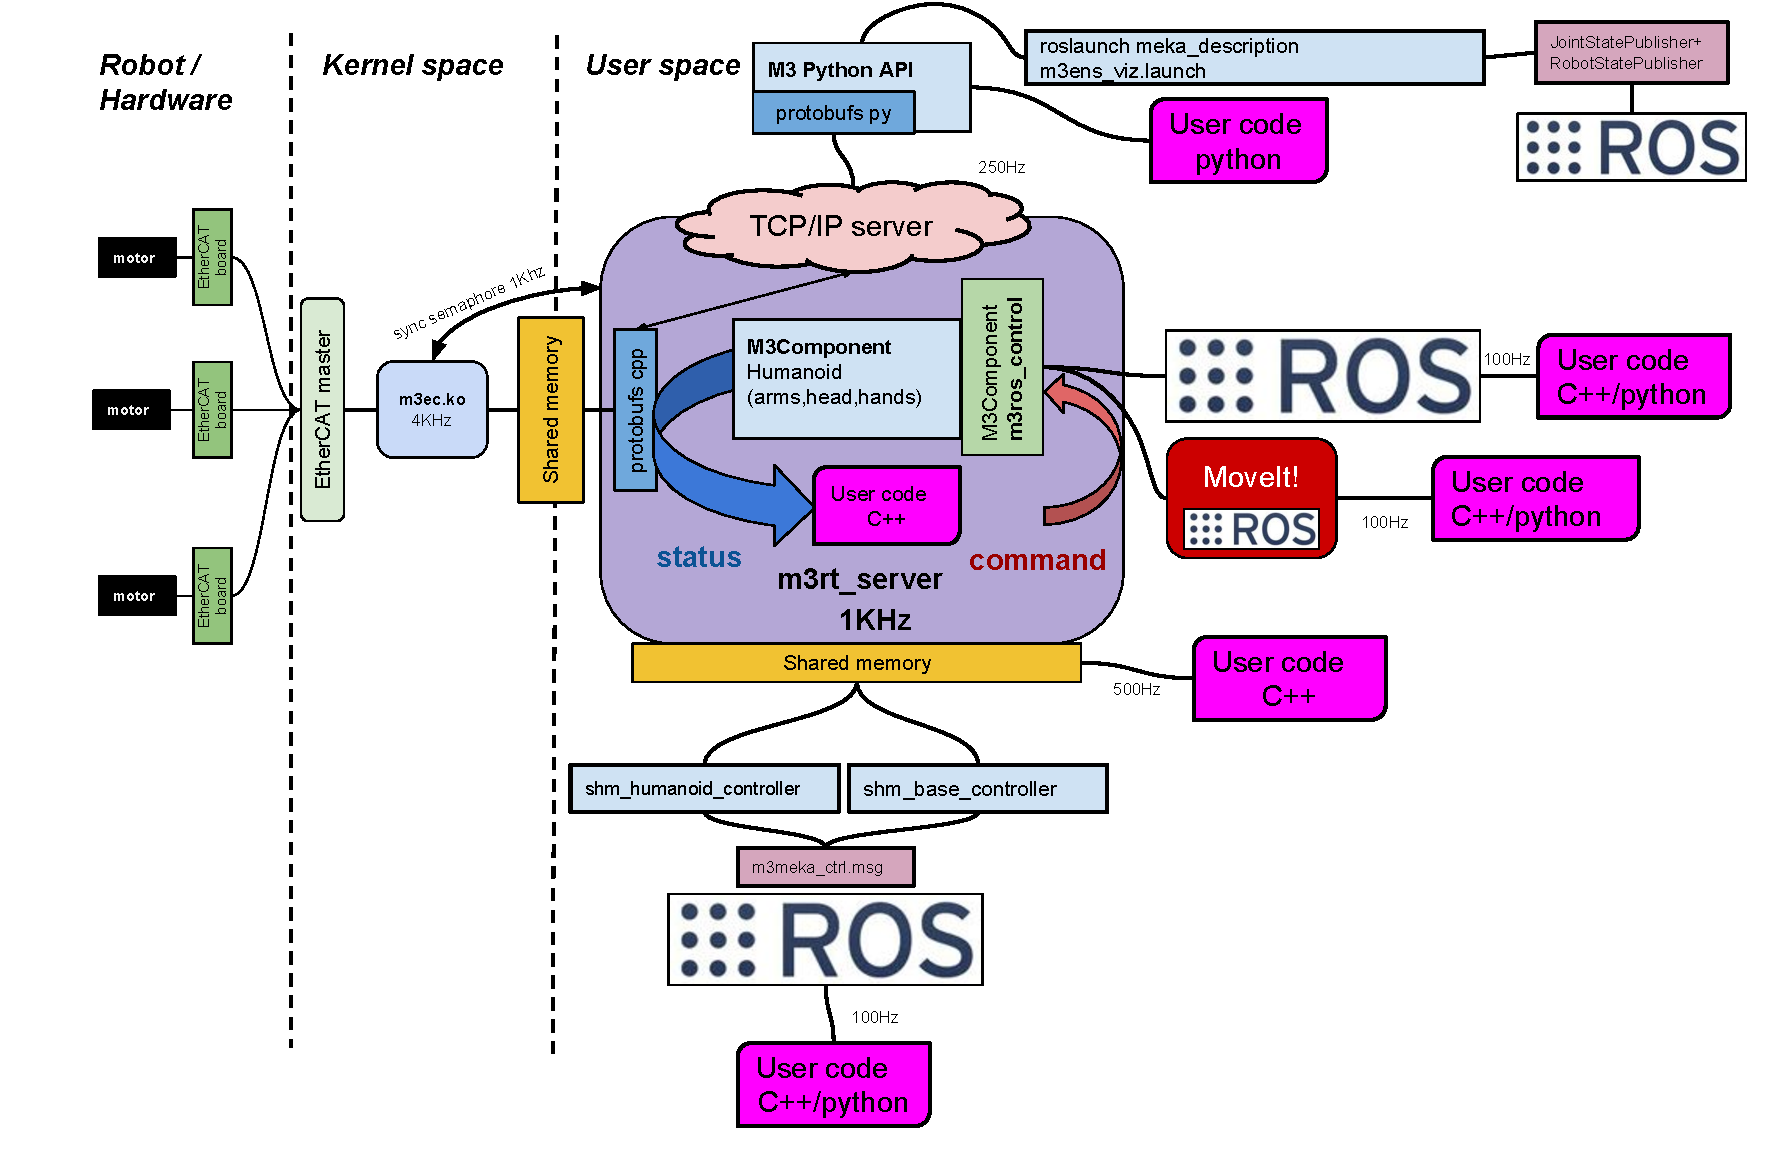
\includegraphics[width=\linewidth]{figs/m3_arch.pdf}
    \caption{Diagrama ilustrativo da arquitetura do robô}
    \label{fig:m3arch}
\end{figure}

\subsection{Controladores Cinemáticos usando Quatérnions Duais}

Os controladores de posição do efetuador foram avaliado a partir da estratégia de discretização dos pontos e frequência de amostragem. Para tal foi reduzido o número de ponto e trajetória foi simplificada para apenas um deslocamento em linha reta de 10cm na vertical. Para primeira análise foi utilizado os controladores implementados anteriormente e foram feitos os seguintes testes:

\begin{enumerate}
    \item Trajetória dividida em 100 pontos, intervalo de 8ms
    \item Trajetória dividida em 100 pontos, intervalo de 100ms
    \item Trajetória dividida em 1000 pontos, intervalo de 8ms
\end{enumerate}

Foi observado que o robô leva um tempo até começar a mexer e um tempo até o controle estabilizar. De modo que está sempre atrasado em relação a referência. Para o período 8ms foram necessárias 25 interações até o robô começar a se mover, com o período de 100 ms o robô começo a se mover já na segunda interação sugerindo um atraso na comunicação de 200ms entre o tempo que o comando é passado via ROS e o tempo que o robô executa o comando.

% Saltos a cada 300 ms

\subsection{API Python}

Para avaliar os controladores de junta de baixo nível foi utilizado a API em Python e a partir dai foram feitos vários teste a partir de comandos de posição para as juntas. A estrutura para envio dos comandos para o robô é diferente, de modo que alguns testes relacionados a comunicação também foram necessários.

\subsubsection{Avaliação do Atraso de Comunicação}
A comunicação com o robô é feita através de uma memória compartilhada. Assim, o primeiro experimento foi levantar o tempo gasto pela instrução \textit{proxy.step()} que atualiza esta memória pegando as medidas dos sensores e informando os comandos para os controladores. Este teste foi feito através avaliando o intervalo de tempo entre cada chamada após sucessivas interações tendo como resultado o valor médio de 16ms entre cada chamada.

\subsubsection{Avaliação do Acumulo do Erro}
Para verificar quanto de erro é acumulado após sucessivas interações foi feito o teste de ler os dados atuais do sensores e passar diretamente para o robô com o objetivo de deixar o robô parado. No entanto foi observado que o braço começou a subir, indicando valores cada vez maiores para os ângulos medidos.

\subsubsection{Identificação da Planta}
Para o experimento de identificação da planta foi aplicado um degrau para cada uma das juntas individualmente. Este teste foi definido a partir dos seguintes passos:

\begin{enumerate}
    \item Começa com a junta na posição 0 graus
    \item Envia o comando para ir para posição 45 graus
    \item Mantém a referência da posição em 45 graus por 2s
    \item Envia o comando para ir para posição 0 graus
    \item Mantém a referência da posição em 0 graus por 2s
\end{enumerate}

Estes passos foram executados 3 vezes para cada uma das juntas. Foi observado um comportamento similar apesar dos motores de cada junta possuírem velocidades de atuação diferente. E novamente o atraso na comunicação pode ser percebido.
